\section{Auswertung}
\label{sec:Auswertung}
\subsection{Bestimmung des RC-Glieds}
Die Messung wird wie in der Duchtführung beschrieben durchgeführt.
Die so erhaltenen Messwerte befinden sich in Tabelle\ref{tab:Messwerte1} :
\begin{table}[H]
    \centering
    \caption{Kondensatorspannung bei fester Frequenz.}
    \label{tab:Messwerte1}
    \begin{tabular}{S[table-format=1.1] S[table-format=2.2] }
        \toprule
        {$t/\si{\milli\second}$} & {$U_C/\si{\volt}$} \\
        \midrule
        0.2 & 14.00 \\
        0.4 & 11.10 \\
        0.6 & 8.64  \\
        0.8 & 6.72  \\
        1.0 & 5.36  \\
        1.2 & 4.08  \\
        1.4 & 3.20  \\
        1.6 & 2.48  \\
        1.8 & 1.92  \\
        2.0 & 1.60  \\
        2.2 & 1.28  \\
        2.4 & 0.96  \\

        \bottomrule
    \end{tabular}
\end{table}

\noindent Die Messwerte werden in der halblogarithmischen Abbildung aufgetragen.
Es wird eine lineare Ausgleichsrechnung, mit Python, durchgeführt und aufgetragen.
Diese hat eine Steigung von $m=\SI{1.228\pm0.008}{\per\milli\second}$
und einen $y$-Achsenabschnitt von $b=(2.890\pm0.005)$.

\begin{figure}
    \centering
    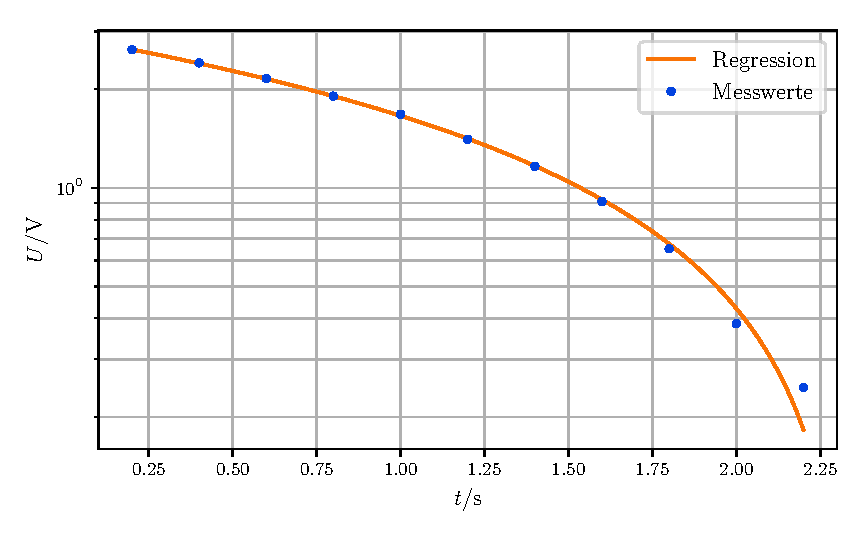
\includegraphics[width=\textwidth]{build/messung1.pdf}
    \caption{Messwerte und Ausgleichsgerade.}
    \label{fig:plot1}
\end{figure}

Die Steigung ist hier $\frac{1}{RC}$ .
Damit ist $RC$ der Kehrwert der Steigung.
\begin{equation*}
  RC=\SI{0.814\pm0.005}{\milli\second}
\end{equation*}
\subsection{Frequenzabhängigkeit der Kondensatorspannung}
Die Messung wird wie in der Durchführung beschrieben ausgeführt.
Die so erhaltenen Messwerte befinden sich in Tabelle\ref{tab:Messwerte2}:
\begin{table}[H]
    \centering
    \caption{Kondensatorspannung bei variabler Frequenz.}
    \label{tab:Messwerte2}
    \begin{tabular}{S[table-format=6.2] S[table-format=2.3] }
        \toprule
        {$f/\si{\hertz}$} & {$U_C/\si{\volt}$} \\
        \midrule
        10.00 & 12.670\\
        12.08 & 12.670\\
        14.94 & 12.750\\
        17.96 & 12.830\\
        20.01 & 12.830\\
        30.00 & 12.860\\
        50.00 & 12.510\\
        80.50 & 11.960\\
        100.00 & 11.480\\
        200.36 & 9.110\\
        300.00  & 7.290\\
        500.00 &  4.790\\
        799.36 &  3.170\\
        1000.00 & 2.530\\
        2000.00 & 1.290\\
        3004.00 & 0.879\\
        3500.00 & 0.768\\
        5000.00 & 0.522\\
        8000.00 & 0.327\\
        10000.00 &  0.263\\
        20000.00 &  0.131\\
        50000.00 &  0.053\\

        \bottomrule
    \end{tabular}
\end{table}
\noindent Die Werte werden in Abbildung aufgetragen.
Durch diese wird eine nichtlineare Ausgleichskurve,mit Gleichung\eqref{eq:gl4}, gezogen.
Die Ausgleichskurve hat die Form:
\begin{equation}
  A(\omega)= \frac{1}{\sqrt{1+\omega^2 m^2}}
\end{equation}
Diese wird mit Python/SciPy aufgetragen.
\begin{figure}[H]
    \centering
    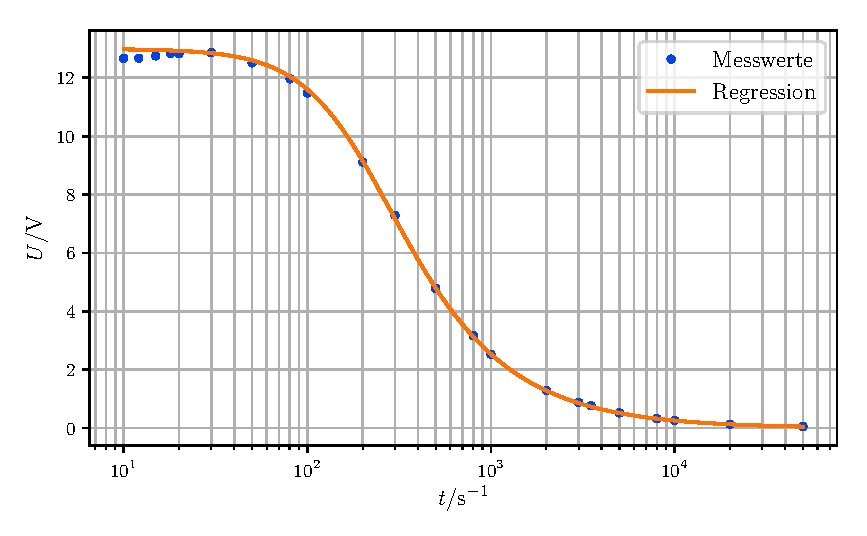
\includegraphics[width=\textwidth]{build/messung2.pdf}
    \caption{Messwerte.}
    \label{fig:plot2}
\end{figure}
\noindent Dabei gilt $m=RC$.
Das so bestimmte RC-Glied hat einen Wert von:
\begin{equation*}
  m = \SI{0.801\pm0.01}{\milli\second}
\end{equation*}
Der gemessene Wert für den Wiederstand des RC-Glieds beträgt:
\begin{equation}
  R = \SI{8.169}{\kilo\ohm}
\end{equation}
%
\subsection{Frequenzabhängigkeit der Phasenverschiebung}
Aus der Messung zur Untersuchung der Frequanzabhängigkeit der Phasenverschiebung zwischen Generator und der Kondensatorspannung ergeben sich die in Tabelle \ref{tab:phase} aufgetragenen Werte. Aus den Messgrößen $a$ und $b$ wird nach Gleichung \eqref{eqn:abphase} der Phasenwinkel $\phi$ berechnen und ist ebenfalls angeführt.
%
\begin{table}[H]
    \caption{Messwerte der Phasenverschiebung.}
    \label{tab:phase}
    \centering
    \begin{tabular}{S[table-format=3.2(0)e0] S[table-format=5.2(0)e0] S[table-format=5.2(0)e0] S[table-format=1.3]}
        \toprule
            {$a/\si{\micro\second}$} & {$b/\si{\micro\second}$} & {$f/\si{\hertz}$} & {$\phi$} \\
        \midrule
        800.00  & 47400.00  & 21.09     & 0.106\\
        800.00  & 19980.00  & 50.08     & 0.252\\
        760.00  & 10000.00  & 100.00    & 0.478\\
        620.00  & 5000.00   & 200.00    & 0.779\\
        520.00  & 3330.00   & 300.00    & 0.981\\
        376.00  & 2000.00   & 500.00    & 1.181\\
        216.00  & 1000.00   & 1000.00   & 1.357\\
        116.00  & 499.84    & 2000.00   & 1.458\\
        68.00   & 285.60    & 3500.00   & 1.496\\
        48.00   & 200.88    & 5000.00   & 1.501\\
        24.00   & 99.84     & 10000.00  & 1.510\\
        12.20   & 50.00     & 20000.00  & 1.533\\
        4.88    & 20.01     & 50000.00  & 1.532\\
        \bottomrule
    \end{tabular}
\end{table}
\noindent
In Abbildung \ref{fig:plot3} sind die Messwerte und eine Theoriekurve nach Gleichung \eqref{eqn:phasetheorie} aufgetragen.
\begin{equation}
    \phi (\omega ) = \arctan (-\omega \, RC) \notag
\end{equation}
Es wird mit Python/SciPy ein Curve-Fit erstellt, der Fit-Parameter ist hierbei $RC$.
\begin{figure}[H]
    \centering
    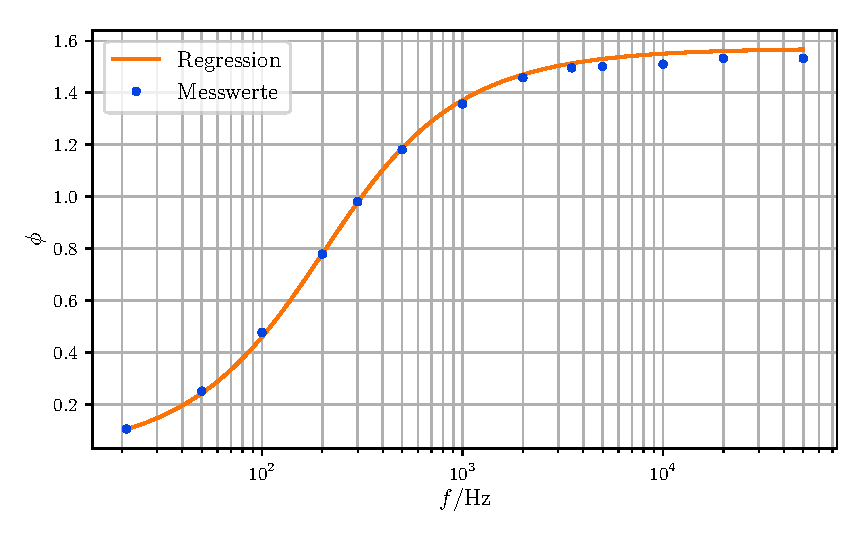
\includegraphics[width=\textwidth]{build/messung3.pdf}
    \caption{Messwerte und Curve-Fit der Phasenverschiebung.}
    \label{fig:plot3}
\end{figure}
\noindent
Es ergibt sich
\begin{equation}
    RC = \SI{0.789\pm0.018}{\milli\second}.
\end{equation}
\noindent
Aus Gleichung \eqref{eqn:phasetheorie} und \eqref{eq:gl4} erhält man eine Relative Amplitude, welche nurnoch vom Phasenwinkel abhängig ist.
\begin{align}
	A(\omega) & = \frac{U_0}{\sqrt{1+\tan^2(\phi)}} \\
	\frac{A(\phi)}{U_0} & = \cos{\phi}
\end{align}
In Abbildung \ref{fig:polar} sind die Theoriekurve der relativen Amplitude und einige Messwertpaare aus Tabellen \ref{tab:phase} und \ref{tab:Messwerte2} in einem Polardiagramm gegen den Phasenwinkel aufgetragen.
\begin{figure}[H]
    \centering
    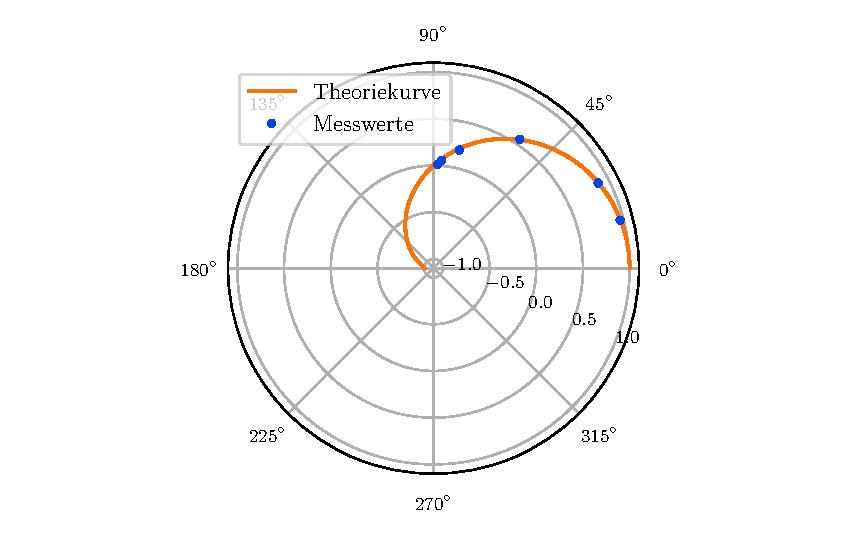
\includegraphics[width=\textwidth]{build/polar.pdf}
    \caption{Relative Amplitude gegen Phasenverschiebung.}
    \label{fig:polar}
\end{figure}
%
\subsection{RC-Glied als Integrator}
\begin{figure}[H]
    \centering
    \begin{minipage}{0.48\textwidth}
        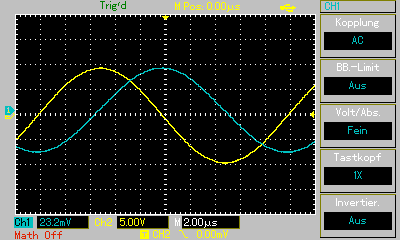
\includegraphics[width=\textwidth]{content/Grafiken/MAP001.png}
        \subcaption{Integration einer Sinusspannung.}
        \label{fig:sinus}
        \vspace{1em}
        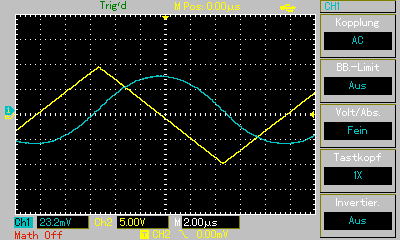
\includegraphics[width=\textwidth]{content/Grafiken/MAP002.png}
        \subcaption{Integration einer Dreieckspannung.}
        \label{fig:dreieck}
        \vspace{1em}
    \end{minipage}
    \hspace*{\fill}
    \begin{minipage}{0.48\textwidth}
        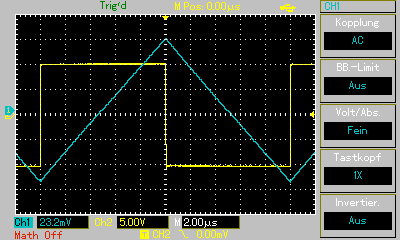
\includegraphics[width=\textwidth]{content/Grafiken/MAP003.png}
        \subcaption{Integration einer Rechteckspannung.}
        \label{fig:rechteck}
        \vspace{1em}
        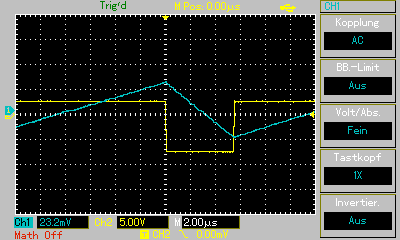
\includegraphics[width=\textwidth]{content/Grafiken/MAP004.png}
        \subcaption{Integration eines PWM-Signals.}
        \label{fig:pwm}
        \vspace{1em}
    \end{minipage}
    \caption{Ursprüngliche und durch den Schwingkreis integrierte Signale.}
\end{figure}
\noindent
In der Abbildung \ref{fig:sinus} ist zu erkennen, wie aus einem negativen Sinussignal ein Cosinussignal entsteht.
Die Dreieckspannung in Abbildung \ref{fig:dreieck} wird auf den linearen Teilstrecken zu Parabeln, welche abwechselnd nach oben und untengeöffnet sind.
Anhand der letzten beiden Abbildungen \ref{fig:rechteck} und \ref{fig:pwm} ist einerseits erkennbar, wie aus einer Stufenfunktion eine streckenweise linear ansteigende und abfallende Funktion wird und andererseits auch, dass durch eine ungleichmäßige Rechteckspannung ein asymmetrisches Signal entsteht.
Aus oben genanntem lässt sich erkennen, dass das RC-Glied in diesem Aufbau als Integrator fungiert.\\
\textbf{Sinusspannung}:
\begin{equation}
  \int - \sin(t) dt = \cos(t)
\end{equation}
\textbf{Dreieckspannug}
\begin{equation}
  \int \begin{dcases}
   \frac{-4}{T}t &  \frac{-T}{4}\leq t \leq \frac{T}{4}\\
   \frac{4}{T}t-2 & \frac{T}{4}\leq t \leq \frac{3T}{4}
 \end{dcases}
 dt = \begin{dcases}
  \frac{-2}{T}t^2 &  \frac{-T}{4}\leq t \leq \frac{T}{4}\\
  \frac{2}{T}t^2-2t & \frac{T}{4}\leq t \leq \frac{3T}{4}
\end{dcases}
\end{equation}
\textbf{Rechteckspannug}
\begin{equation}
  \int \begin{dcases}
   -1 & 0 \leq t \leq \frac{T}{2}\\
    1 & \frac{T}{2}\leq t \leq T
 \end{dcases}
 dt = \begin{dcases}
    -t &  0 \leq t \leq \frac{T}{2}\\
     t & \frac{T}{2}\leq t \leq  T
   \end{dcases}
\end{equation}
\textbf{PWM-Signal}
\begin{equation}
  \int \begin{dcases}
   -\frac{a}{T} & 0 \leq t \leq \frac{T}{a}\\
    \frac{1-a}{T} & \frac{T}{a}\leq t \leq T
 \end{dcases}
 dt = \begin{dcases}
    -\frac{a}{T}t &  0 \leq t \leq \frac{T}{a}\\
     \frac{1-a}{T}t & \frac{T}{a}\leq t \leq  T
   \end{dcases}
\end{equation}
